\expandafter\newcommand\csname dataGBmetrictab\endcsname{
\begin{table}[H]
\begin{tabular}
{| 
 p{\dimexpr0.2\textwidth-2\tabcolsep-\arrayrulewidth\relax}| 
 p{\dimexpr0.2\textwidth-2\tabcolsep-\arrayrulewidth\relax}| 
 p{\dimexpr0.2\textwidth-2\tabcolsep-\arrayrulewidth\relax}| 
 p{\dimexpr0.2\textwidth-2\tabcolsep-\arrayrulewidth\relax}| 
 p{\dimexpr0.2\textwidth-2\tabcolsep-\arrayrulewidth\relax}| 
}\hline 
\textbf{} &\textbf{f1-score} &\textbf{precision} &\textbf{recall} &\textbf{support} \\ \hline 
CANDIDATE &0.658 &0.737 &0.594 &170.0 \\ \hline 
CONFIRMED &0.859 &0.824 &0.896 &241.0 \\ \hline 
FALSE POSITIVE &0.945 &0.931 &0.959 &391.0 \\ \hline 
accuracy &0.863 &0.863 &0.863 &0.863 \\ \hline 
macro avg &0.82 &0.831 &0.816 &802.0 \\ \hline 
weighted avg &0.858 &0.858 &0.863 &802.0 \\ \hline 
\end{tabular} 
\end{table}
}
\begin{figure}[H]
                \begin{mdframed}[linecolor=green]
                \centering
                \begin{subfigure}{.49\textwidth}
                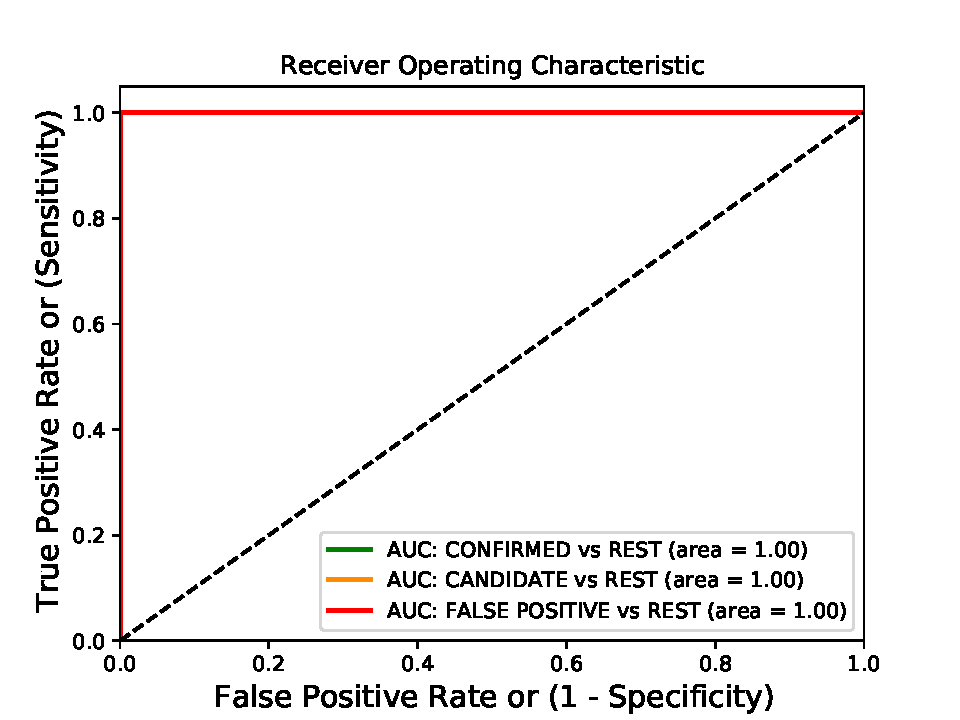
\includegraphics[width = 1\textwidth]{data/GB_overfit_roc.pdf}
                \end{subfigure}
                \begin{subfigure}{.49\textwidth}
                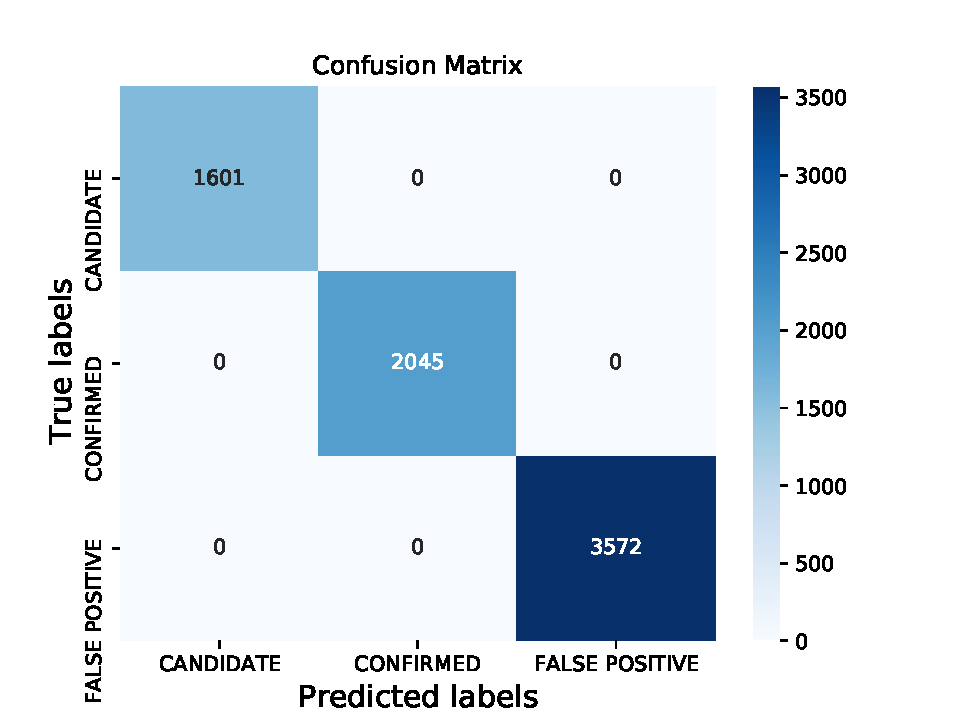
\includegraphics[width = 1\textwidth]{data/GB_overfit_cm.pdf}
                \end{subfigure}
                \begin{subfigure}{.49\textwidth}
                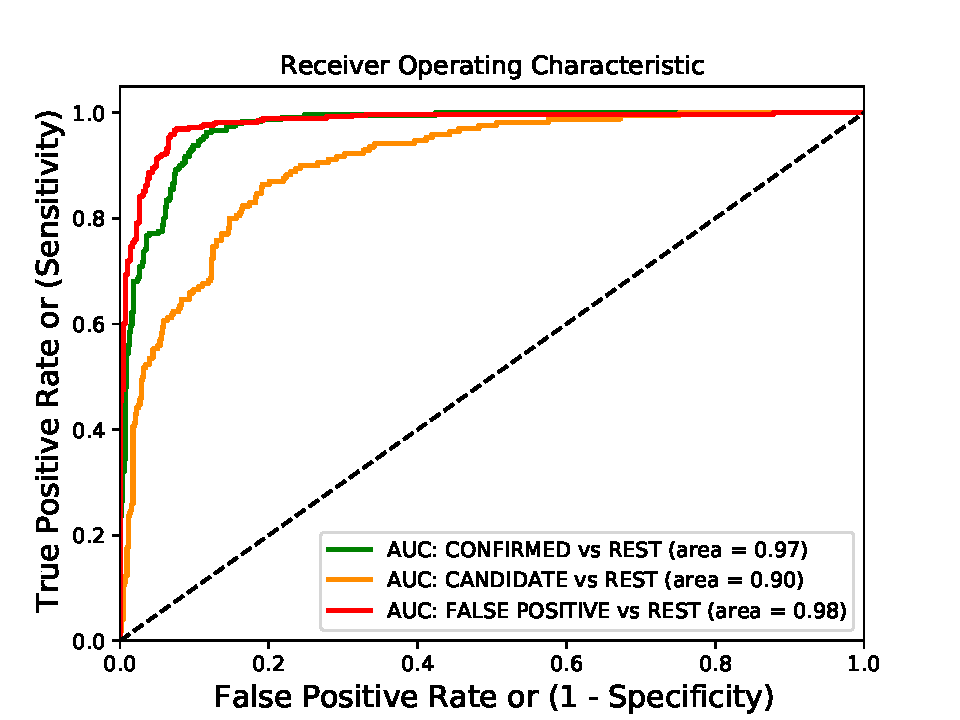
\includegraphics[width = 1\textwidth]{data/GB_roc.pdf}
                \end{subfigure}
                \begin{subfigure}{.49\textwidth}
                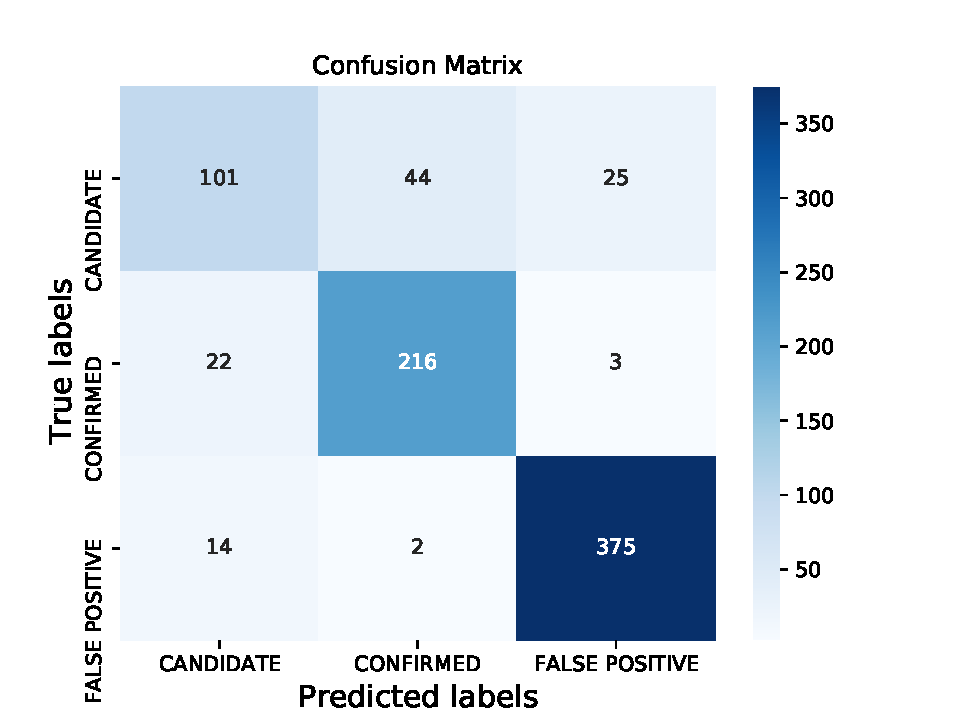
\includegraphics[width = 1\textwidth]{data/GB_cm.pdf}
                \end{subfigure}
                \begin{subfigure}{1\textwidth}
                \csname dataGBmetrictab\endcsname
                \end{subfigure}
                \caption{GB: Top Row: overfit test. Middle and bottom row test data}
                \label{fig:data/GB_roc}
                \end{mdframed}
                \end{figure}